
\documentclass[10pt,oneside]{report}

\setcounter{secnumdepth}{4}
\setcounter{tocdepth}{4}

%%%%%%%%%%%%%%%%%%%%%%%%%%%%%%%%%%%%%%%%%%%%%%%%%%%%
\usepackage[english]{babel}
\usepackage[utf8]{inputenc}
\usepackage[T1]{fontenc}
\usepackage{lmodern}
\usepackage{hyperref} % must be loaded before glossaries-extra
\usepackage{setspace}
% bibliography
\usepackage[hyperref=true,backref=true,backend=biber,maxbibnames=9,maxcitenames=2,style=numeric,citestyle=numeric,sorting=none]{biblatex}

\usepackage{adjustbox}
\usepackage{algorithm}
\usepackage{algpseudocode}
\usepackage{amsfonts}
\usepackage{amsmath}
\usepackage{amssymb}
\usepackage{bm}
\usepackage{booktabs}
\usepackage[labelfont=bf]{caption}
\usepackage{csquotes}
\usepackage{enumitem}

\usepackage{fancyhdr}

\usepackage[a4paper, 
left=2.54cm, 
right=2.54cm, 
top=2.54cm, 
bottom=2.54cm, 
bindingoffset=0.7cm]{geometry}

\usepackage[%
    toc,
    %record,
    symbols,
    nonumberlist,
    nogroupskip,
]{glossaries-extra}

\usepackage{graphicx}
\usepackage{listings}
\usepackage{lipsum}
\usepackage{makecell}
\usepackage{mathtools}
\usepackage{mfirstuc}
\usepackage[final,verbose=silent]{microtype}
\usepackage{multirow}
\usepackage{nicefrac}
\usepackage{ragged2e}
\usepackage{siunitx}
\usepackage{svg}
\usepackage{tabularx}
\usepackage{textcomp}
\usepackage{tikz}
\usetikzlibrary{positioning,arrows.meta,shapes.geometric,fit,backgrounds,calc}
\usepackage{url}
\usepackage{verbatim}
\usepackage{xcolor}

\usepackage{titlesec}
\usepackage{longtable}
\usepackage{subcaption}
\usepackage{threeparttable}


\input{common/package_config}

\input{common/new_commands}

% change this configuration with your info
% if you need fewer or more supervisors you have to change \relatore command by adding or removing lines in the table in toptesi_config
\newcommand{\thesistitle}{An Open-Source Framework for the hydroelastic analysis of composite hydrofoils} % title of the thesis
\newcommand{\thesisuniversitylogo}{images/polito_logo_2021_blu} % choose your logo
\newcommand{\thesiscandidatename}{Lorenzo}
\newcommand{\thesiscandidatesurname}{Valle}

\newcommand{\thesissupervisoronetitle}{prof.}
\newcommand{\thesissupervisoronename}{Pietro}
\newcommand{\thesissupervisoronesurname}{Casalone}

\newcommand{\thesissupervisortwotitle}{prof.}
\newcommand{\thesissupervisortwoname}{Mauro}
\newcommand{\thesissupervisortwosurname}{Bonfanti}

\newcommand{\thesissupervisorthreetitle}{ing.}
\newcommand{\thesissupervisorthreename}{Davide}
\newcommand{\thesissupervisorthreesurname}{Tagliapietra}

\newcommand{\thesissupervisorfourtitle}{ing.}
\newcommand{\thesissupervisorfourname}{Luca}
\newcommand{\thesissupervisorfoursurname}{Valsecchi}

\newcommand{\thesissupervisorfivetitle}{ing.}
\newcommand{\thesissupervisorfivename}{Paolo}
\newcommand{\thesissupervisorfivesurname}{Motta}

\newcommand{\thesisdate}{MARCH 2026}
\newcommand{\thesiscourse}{MECHANICAL ENGINEERING}

\newcommand{\thesisuniversity}{POLITECNICO DI TORINO}

\newcommand{\thesislevel}{MASTER} % master or bachelor

\newcommand{\thesiscandidatetext}{Candidate}
\newcommand{\thesissupervisortext}{Supervisors}
\newcommand{\thesisexternalsupervisortext}{External Supervisors}
\newcommand{\thesisdepartment}{Department of Mechanical and Aerospace Engineering}


\input{common/font_config.tex}

\addbibresource{bibliography.bib}
% Additional bibliography file (chapter-specific or recently added refs)
\addbibresource{common/bibliography_extra.bib}

% Load nomenclature definitions
\input{nomenclature.tex}
\makeglossaries

\setlength{\headheight}{14pt}

% Customize chapter formatting to remove "Chapter X"
\titleformat{\chapter}[display]
  {\normalfont\huge\bfseries}  % Format for chapter title
  {}  % Empty - removes "Chapter X"
  {0pt}  % Space between label and title
  {\LARGE}  % Format for the title text
\titlespacing*{\chapter}
  {0pt}  % Left margin
  {0pt}  % Space before the title (reduced from default ~50pt)
  {15pt}  % Space after the title (reduced from default ~40pt)

% Reduce spacing in itemize and enumerate environments
\setlist[itemize]{itemsep=2pt, parsep=0pt, topsep=5pt}
\setlist[enumerate]{itemsep=2pt, parsep=0pt, topsep=5pt}

% Available font sizes:
%\tiny
%\scriptsize
%\footnotesize
%\small
%\normalsize
%\large
%\Large          % <-- Good for chapter titles
%\LARGE
%\huge
%\Huge           % <-- Default, very large

\begin{document}

\pagestyle{fancy}
\fancyhf{}
\fancyhead[C]{\itshape \leftmark}  % Titolo del capitolo in corsivo
\fancyfoot[C]{\thepage}  % Numero di pagina centrato in basso
% Personalizza \chaptermark per mostrare solo il titolo, senza "Chapter X"
\renewcommand{\chaptermark}[1]{\markboth{#1}{}}
\renewcommand{\headrulewidth}{0.4pt}  % Optional: add header line

\input{common/config}
\input{common/frontpage.tex} % custom frontpage

% Insert blank page after frontpage
\newpage
\thispagestyle{empty}
\mbox{}  % This creates an empty box to force the page to exist
\newpage

%\frontmatter
\pagenumbering{Roman}

%abstract if needed
\begin{abstract}


%\fancyhf{} % clear all header and footer fields
%\fancyhead[RO,R]{\thepage} %RO=right odd, RE=right even
%\renewcommand{\headrulewidth}{0pt}

%\begin{center}
%    %\Large
%    %\textbf{Thesis Title}
%    %
%    %\vspace{0.4cm}
%    %
%    %\vspace{0.4cm}
%    %\textbf{Thesis Author}
%    
%    \vspace{0.9cm}
%    \textbf{Abstract}
%    
%\end{center}

The increasing integration of composite materials into marine lifting surfaces, such as hydrofoils and turbine blades, 
is unlocking new opportunities for weight reduction and structural efficiency. However, this trend amplifies the need for reliable prediction 
of unsteady hydrodynamic behaviour and coupled hydro-elastic instabilities, with flutter remaining one of the most critical challenges. 
Most available numerical tools are either accurate but computationally expensive or rely on oversimplified modelling that fails to capture the complex 
coupling between hydrodynamics, structural anisotropy, and dynamic stability.
This work introduces a comprehensive framework that directly addresses these limitations. 
The toolchain integrates four key components into a unified workflow: a finite-element pre-processor for generating fully coupled 
six degrees of freedom beam models; a dynamic beam solver for time-domain structural response; a Doublet Lattice Method implementation for unsteady 
hydrodynamic load prediction; and a robust P-K analysis module featuring automatic mode tracking. 
Together, these modules enable accurate coupling of structural and hydrodynamic phenomena, delivering a comprehensive toolset for frequency-domain response 
evaluation and instability prediction.
The proposed framework, using reduced-order modelling, achieves high computational efficiency while maintaining accuracy.
This balance between fidelity and cost-effectiveness makes the tool ideal for early-stage design, parametric studies, and optimisation tasks.
The methodology and software architecture are described in detail and validated against experimental data for a hydrofoil with heterogeneous cross-sections.
Results show very good agreement, confirming the tool’s capability to capture coupled fluid–structure dynamics and accurately predict critical flutter conditions.

\end{abstract}

% Blank page after abstract
\clearpage
\thispagestyle{empty}
\mbox{}
\clearpage

%\ringraziamenti
% acknowledgements

ACKNOWLEDGMENTS

\vspace*{5\baselineskip}

\begin{flushright}
    \textit{a due persone speciali, a due persone che sanno gioire sempre, che mi insegnano ogni giorno, che mi guardano con occhi critici ma pieni di orgoglio, che faticano in silenzio e che mi vogliono bene. A mio papà Andrea e mia mamma Angelica.}
\end{flushright}


\tableofcontents

\listoffigures

\listoftables

% Nomenclature page
\printunsrtglossary[style=long,title=Nomenclature,type=symbols]

\input{common/post_summary_config.tex}

\newpage
\pagenumbering{arabic}
% list here all the chapters
\chapter{Introduction}
\section{Context and motivation}
In the last few years, the use of slender load-bearing profiles in hydrodynamic environments, such as hydrofoils for racing yachts,
marine propulsion systems and renewable energy devices, has grown significantly.
The adoption of lightweight structures, often made of composite materials, allows for improving overall system efficiency,
but it makes such components more sensitive to aero-hydro-elastic undesired phenomena, particularly flutter.

Flutter represents a form of self-excited dynamic instability, where the interaction between structural rigidity, 
inertias and fluid-dynamic loads leads to increasing amplitude oscillations.
For a hydrofoil, the onset of flutter can lead to loss of performance, structural damage or collapse, with possible
relevant safety consequences, reliability impacts and operational costs.

It thus becomes essential to develop analysis instruments able to prevent, during the design phase, the onset of these instabilities,
guiding geometrical, material and mass distribution choices.

High-fidelity approaches based on computational fluid dynamics coupled with complex structural models guarantee high accuracy of the phenomenon,
but they are often computationally expensive and difficult to integrate into iterative design cycles.
On the other hand, aeroelastic reduced-order methods, which combine beam models with unsteady potential aerodynamics,
offer an advantageous compromise between accuracy and computational cost. Naturally, the workflow chain must be defined coherently, verified and reproducible.

This thesis fits into this context, aiming to develop a modular numerical procedure for analyzing flutter of slender wings, 
with particular attention to hydrofoils.

\section{Current challenges}
Extensive literature covers aeroelasticity of wings in aerodynamic environments and, increasingly, of hydrofoils in hydrodynamic flows. 
However, several recurring critical gaps are observed:

\begin{itemize}
    \item absence of an integrated workflow spanning from realistic section definition (materials, layup, shear center and mass center locations) to flutter prediction in a coherent manner;
    \item limited availability of readily integrable tools combining:
    \begin{itemize}
        \item flexible parametrization of geometry and material properties,
        \item generation of stiffness and mass properties for composite sections,
        \item a dedicated flexible beam solver,
        \item a consolidated, unsteady panel aerodynamic model,
        \item a flutter solver based on standard industrial methods;
    \end{itemize}
    \item fragmented documentation, hindering result reuse and adoption in preliminary design workflows.
\end{itemize}

These gaps motivate the development of a transparent computational environment, verified against known benchmarks and readily extensible 
to diverse wing and hydrofoil configurations.

\section{Objectives of this thesis}
The overall objective of this thesis is to define, implement, and validate a modular numerical procedure for analyzing flutter of slender wing structures 
in fluid environments, with particular reference to hydrofoils, based on the seamless coupling of structural, aerodynamic, and hydrodynamic analysis modules.

In particular, the work aims to:
\begin{enumerate}
    \item define a \textbf{standardized input model} for describing geometry, materials and layup of wing sections,
    \item build a \textbf{modular computational chain} using the consolidated \textbf{SONATA/ANBA4} tool to generate cross-sectional structural matrices and the associated one-dimensional Euler-Bernoulli beam model,
    \item implement and verify a \textbf{custom FEM beam solver} for static and modal analysis of equivalent beams, comparing results with literature solutions and reference cases (Timoshenko beams, cantilevers, and modal verification),
    \item develop a comprehensive \textbf{aerodynamic and hydrodynamic modeling framework} integrating the \textbf{Doublet Lattice Method} (via \textbf{PanelAero}) for unsteady forces, \textbf{Rational Function Approximation} (RFA) for frequency-dependent aerodynamic matrices, and a \textbf{hybrid DLM-BEM approach} combining DLM with \textbf{Capytaine BEM} to capture three-dimensional added-mass effects in water,
    \item define a coherent \textbf{coupling strategy} between the aerodynamic/hydrodynamic grid and structural finite-element nodes, with explicit treatment of both aeroelastic (air) and hydroelastic (water) environments,
    \item implement a \textbf{flutter solver} based on the industrial-standard \textbf{p--k method}, including automatic mode tracking and eigenvalue convergence criteria,
    \item \textbf{integrate all modules} into a coherent, reproducible, and openly documented computational workflow,
    \item \textbf{verify and validate} each module and the complete procedure against established benchmarks (Goland wing for aeroelasticity, NACA0003 for hydroelasticity, literature data),
    \item apply the \textbf{end-to-end procedure} to realistic \textbf{hydrofoil case studies} (wing01 flexible wing and tnz\_multibody assembly), evaluating the effect of structural and modeling parameters on dynamic behavior and flutter boundary conditions.
\end{enumerate}

\begin{figure}[h]
    \centering
    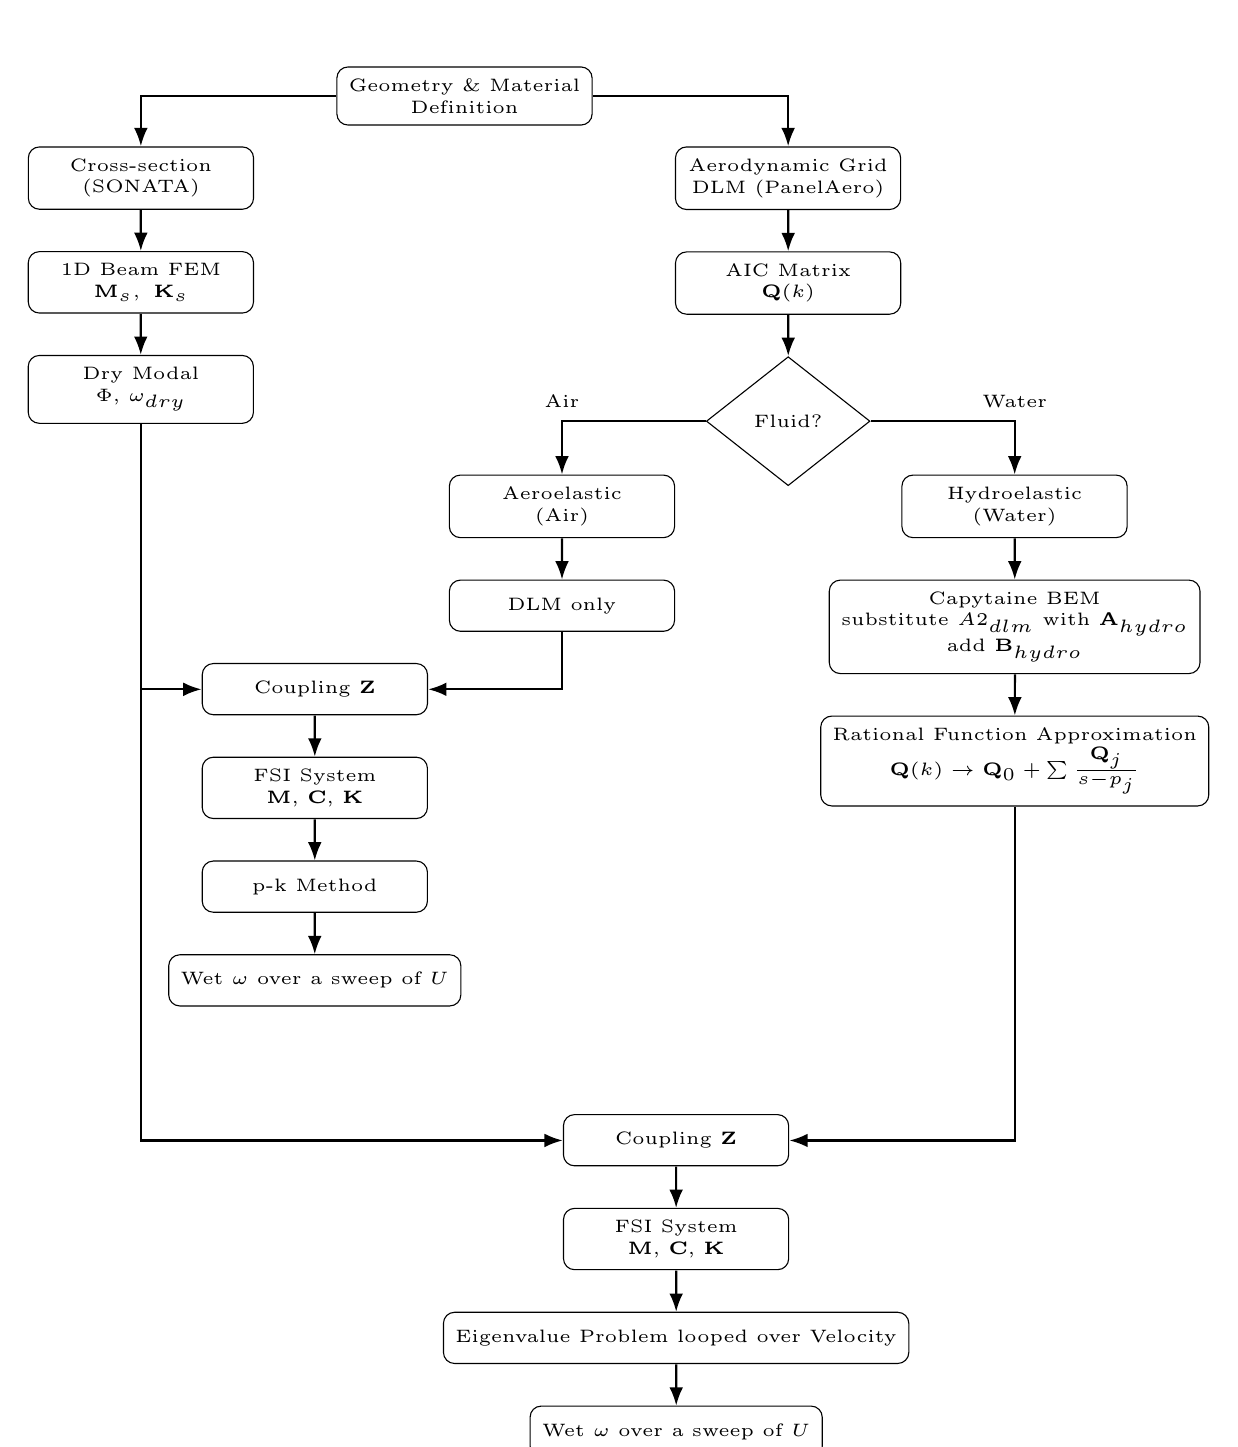
\begin{tikzpicture}[
        >=LaTeX,
        node distance=0.9cm,
        scale=1.3,
        transform shape,
        block/.style={
            rectangle,
            draw,
            rounded corners,
            align=center,
            minimum width=2.2cm,
            minimum height=0.5cm,
            font=\tiny
        },
        line/.style={->, thick, line width=0.8pt},
        decision/.style={
            diamond,
            draw,
            align=center,
            minimum width=1.6cm,
            minimum height=0.6cm,
            font=\tiny
        }
    ]

    % TOP: GEOMETRY AND INPUTS
    \node[block] (geom) {Geometry \& Material\\Definition};
    
    % LEFT BRANCH: STRUCTURAL PATH
    \node[block, below left=0.2cm and 0.8cm of geom] (sonata) {Cross-section\\(SONATA)};
    \node[block, below=0.4 of sonata] (fem) {1D Beam FEM\\$\mathbf{M}_s,\ \mathbf{K}_s$};
    \node[block, below=0.4 of fem] (dry) {Dry Modal\\$\Phi$, $\omega_{dry}$};

    % RIGHT BRANCH: AERODYNAMIC PATH (DLM)
    \node[block, below right=0.2cm and 0.8cm of geom] (aero) {Aerodynamic Grid\\DLM (PanelAero)};
    \node[block, below=0.4 of aero] (aic) {AIC Matrix\\$\mathbf{Q}(k)$};

    % Decision point: Aeroelastic vs Hydroelastic
    \node[decision, below=0.4 of aic] (decide) {Fluid?};
    
    % AEROELASTIC PATH (left branch from decision)
    \node[block, below left=0.2cm and 0.7cm of decide] (aero_path) {Aeroelastic\\(Air)};
    \node[block, below=0.4 of aero_path] (aero_matrices) {DLM only};

    % CONVERGENCE POINT: Both paths merge
    \node[block, below left=0.3cm and 0.2 cm of aero_matrices] (coupling1) {Coupling $\mathbf{Z}$};

    % HYDROELASTIC PATH (right branch from decision)
    \node[block, below right=0.2cm and 0.7cm of decide] (hydro_path) {Hydroelastic\\(Water)};
    \node[block, below=0.4 of hydro_path] (bem) {Capytaine BEM\\ substitute $A2_{dlm}$ with $\mathbf{A}_{hydro}$ \\ add $\mathbf{B}_{hydro}$};
    \node[block, below=0.4 of bem] (RFA) {Rational Function Approximation\\$\mathbf{Q}(k) \to \mathbf{Q}_0 + \sum \frac{\mathbf{Q}_j}{s - p_j}$};

    % CONVERGENCE POINT: Both paths merge
    \node[block, below left=3cm and 0.3 cm of RFA] (coupling2) {Coupling $\mathbf{Z}$};
    
    % SYSTEM ASSEMBLY
    \node[block, below=0.4 of coupling1] (wet1) {FSI System\\$\mathbf{M}$, $\mathbf{C}$, $\mathbf{K}$};
    \node[block, below=0.4 of wet1] (flutter1) {p-k Method};
    \node[block, below=0.4 of flutter1] (output1) {Wet $\omega$ over a sweep of $U$};

    % SYSTEM ASSEMBLY
    \node[block, below=0.4 of coupling2] (wet2) {FSI System\\$\mathbf{M}$, $\mathbf{C}$, $\mathbf{K}$};
    \node[block, below=0.4 of wet2] (flutter2) {Eigenvalue Problem looped over Velocity};
    \node[block, below=0.4 of flutter2] (output2) {Wet $\omega$ over a sweep of $U$};

    % ============================================================
    % CONNECTIONS: Structural path
    % ============================================================
    \draw[line] (geom) -| (sonata);
    \draw[line] (sonata) -- (fem);
    \draw[line] (fem) -- (dry);
    \draw[line] (dry) |- (coupling1);
    \draw[line] (dry) |- (coupling2);

    % ============================================================
    % CONNECTIONS: Aerodynamic path (DLM + RFA)
    % ============================================================
    \draw[line] (geom) -| (aero);
    \draw[line] (aero) -- (aic);
    \draw[line] (aic) -- (decide);

    % ============================================================
    % CONNECTIONS: Aeroelastic vs Hydroelastic decision
    % ============================================================
    \draw[line] (decide) -| (aero_path) node[midway, above, font=\tiny] {Air};
    \draw[line] (decide) -| (hydro_path) node[midway, above, font=\tiny] {Water};

    % ============================================================
    % CONNECTIONS: Aeroelastic branch
    % ============================================================
    \draw[line] (aero_path) -- (aero_matrices);
    \draw[line] (aero_matrices) |- (coupling1);

    % ============================================================
    % CONNECTIONS: System assembly and solution
    % ============================================================
    \draw[line] (coupling1) -- (wet1);
    \draw[line] (wet1) -- (flutter1);
    \draw[line] (flutter1) -- (output1);

    % ============================================================
    % CONNECTIONS: Hydroelastic branch
    % ============================================================
    \draw[line] (hydro_path) -- (bem);
    \draw[line] (bem) -- (RFA);
    \draw[line] (RFA) |- (coupling2);

    % ===========================================================
    % CONNECTIONS: System assembly and solution
    % ============================================================
    \draw[line] (coupling2) -- (wet2);
    \draw[line] (wet2) -- (flutter2);
    \draw[line] (flutter2) -- (output2);

    \end{tikzpicture}
    \caption{Unified workflow for aeroelastic and hydroelastic flutter analysis.}
    \label{fig:aeroelastic_workflow}
\end{figure}

To ensure the validity of the work, each custom-built module and the entire workflow are validated both analytically
and with reference benchmark cases.

The unified workflow for aeroelastic and hydroelastic flutter analysis is represented in Figure \ref{fig:aeroelastic_workflow}. The scheme illustrates the hybrid DLM-BEM approach tailored for hydrofoil design: 

\begin{itemize}
    \item The \textbf{left branch} develops structural properties: geometry and material definitions are processed through SONATA/ANBA4 to generate cross-sectional matrices, which are then assembled into a one-dimensional finite-element beam model. A ``dry'' modal analysis (without fluid loading) is performed to extract the structural eigenvalues and eigenvectors serving as the baseline for aeroelastic coupling.
    \item The \textbf{right branch} develops aerodynamic matrices: the aerodynamic grid is discretized for the Doublet Lattice Method (PanelAero), the Aerodynamic Influence Coefficient (AIC) matrix $\mathbf{Q}(k)$ is computed as a function of reduced frequency, and Rational Function Approximation is applied to obtain frequency-independent aerodynamic coefficients suitable for flutter analysis.
    \item A \textbf{decision point} routes the analysis to either the \textbf{aeroelastic path} (air environment, using DLM exclusively) or the \textbf{hydroelastic path} (water environment, combining DLM with Capytaine BEM corrections). The hybrid approach eliminates the thin-wing approximation error inherent in DLM by replacing the asymptotic added-mass term with Capytaine's three-dimensional boundary-element calculation $\mathbf{A}_{hydro}(\infty)$.
    \item Both paths converge at the \textbf{coupling matrix} $\mathbf{Z}$, where structural and aerodynamic/hydrodynamic terms are assembled into a unified FSI system with mass $\mathbf{M}$, damping $\mathbf{C}$, and stiffness $\mathbf{K}$ matrices.
    \item The \textbf{p-k method} solves for the stability characteristics (eigenvalues and eigenvectors) across a sweep of velocities, identifying the flutter boundary where damping transitions from positive (stable) to negative (unstable).
    \item The output is the complete flutter envelope: ``wet'' natural frequencies and damping ratios plotted as functions of flow velocity.
\end{itemize}

\newpage
\section{Document structure}
The remainder of this document is organized as follows:

Chapter 2 (\textit{Structural Modeling and FEM Analysis}) introduces the theoretical foundations of beam structural modeling for slender structures, the development of cross-sectional properties, assembly of finite-element matrices, and the concept of ``dry'' modal analysis without fluid coupling.

Chapter 3 (\textit{Aeroelastic and Hydroelastic Modeling}) establishes the distinction between aeroelastic (air) and hydroelastic (water) environments, describes the aerodynamic and hydrodynamic force models based on the Doublet Lattice Method (DLM) and Boundary Element Method (BEM), introduces Rational Function Approximation (RFA) for frequency-dependent aerodynamic matrices, and defines the coupling strategy between structural and fluid domains. A hybrid DLM-BEM approach is presented for hydrofoil applications to capture three-dimensional added-mass effects while maintaining computational efficiency.

Chapter 4 (\textit{Flutter Analysis: The p-k Method}) details the mathematical formulation and numerical implementation of the p--k method, including the nested outer loop (velocity sweep, altitude, Mach number) and inner loop (mode-by-mode iterative solution with reduced frequency updating). The chapter includes detailed flowcharts, convergence criteria, and mode-tracking algorithms essential for automated flutter identification.

Chapter 5 (\textit{Verification and Validation}) presents systematic validation of the aeroelastic and hydroelastic frameworks through sensitivity studies, grid convergence analyses, and benchmark comparisons. The Goland wing flutter test case is used as the primary aeroelastic reference, while the NACA0003 hydrofoil provides hydroelastic validation. Each stage of the pipeline is verified against established analytical and numerical results.

Chapter 6 (\textit{Hydrofoil Case Study}) demonstrates the complete end-to-end application of the developed workflow to realistic hydrofoil structures. The chapter covers two primary applications: the \texttt{wing01} flexible composite hydrofoil (examining isolated wing dynamics) and the \texttt{tnz\_multibody} assembly (representing a practical racing-yacht foil system). Results include dry and wet modal characteristics, flutter boundaries, and parametric sensitivity studies.

Chapter 7 (\textit{Discussion, Conclusion and Further Work}) synthesizes the results, provides critical assessment of the developed framework, discusses model limitations and design implications, and proposes future developments including complete Rational Function Approximation, viscous effects modeling, cavitation analysis, and experimental validation.

\chapter{Structural Modeling and FEM Analysis}
\label{chap:structure}

\section{Description of the physical problem}
This work is dedicated to the study of dynamic behavior of load-bearing slender structures immersed in a fluid flow,
with particular reference to wings and hydrofoils. Such structures are characterized by high geometric slenderness, comparable flexural
and torsional stiffness and marked interaction with the surrounding fluid.

When a deformable structure is immersed in a flow, the aerodynamic or hydrodynamic forces acting on it depend not only
on the instantaneous geometric configuration, but also on the motion of the structure itself. Displacements and rotations modify
the velocity field of the fluid, which in turn generates pressure variations responsible for additional loads on the structure. This
feedback mechanism constitutes the foundation of fluid-structure interaction.

Under certain operating conditions, the interaction between elastic, inertial and fluid forces can lead to dynamic instability phenomena.
Among these, flutter represents one of the most relevant issues from a design perspective, as it manifests as a self-excited oscillation
that can rapidly lead to response levels incompatible with structural integrity.

The objective of aeroelastic analysis, therefore, is the prediction of conditions in which such instabilities can arise, starting from a physically
coherent description of the structure, fluid and their coupling. In the present work, the problem is addressed in the context of linear dynamics, 
assuming small displacements and linear elastic behavior of the structure.

\section{General equation of aeroelastic motion}
The dynamic behavior of a deformable structure immersed in a flow can be described by a set of differential equations
that express the equilibrium between inertial, elastic, dissipative and fluid forces. Introducing a vector of generalized coordinates $\mathbf{q}(t)$,
which represents the dynamic state of the structure, the equation of motion can be written in general form:
\begin{equation}
    \mathbf{M_s} \ddot{\mathbf{q}}(t) + \mathbf{C_s} \dot{\mathbf{q}}(t) + \mathbf{K_s} \mathbf{q}(t) = \mathbf{F_{aero}(\mathbf{q(t),\dot{q}(t),U_{{\infty}}(t)})}
    \label{eq:general_motion_equation}
\end{equation}
where:
\begin{itemize}
    \item $\mathbf{M_s}$ is the structural mass matrix;
    \item $\mathbf{C_s}$ is the structural damping matrix;
    \item $\mathbf{K_s}$ is the elastic stiffness matrix;
    \item $\mathbf{F_{aero}}$ represents the vector of unsteady aerodynamic or hydrodynamic forces;
    \item $\mathbf{U_{{\infty}}}$ is the undisturbed flow velocity vector.
\end{itemize}

Equation~\ref{eq:general_motion_equation} highlights how the aeroelastic problem is intrinsically coupled: the fluid load term depends on
the motion of the structure and, at the same time, contributes to modifying its dynamic response. Unlike classical structural problems, in which external forces
are prescribed, in this context they constitute a function of the dynamic state of the system.

In the present work, attention is directed toward small-amplitude harmonic motion regimes, for which it is possible to linearize the fluid term with respect
to generalized coordinates and their derivatives. This assumption allows us to reduce the problem to the search for exponential solutions and
to analyze their stability through eigenvalue techniques.

The equation of motion represents the heart of aeroelastic analysis and serves as the conceptual reference for the entire thesis. In subsequent chapters,
each term will be defined, modeled and physically interpreted, always maintaining explicit the link between theoretical formulation and the physical reality of the phenomenon.

\section{Reference system and kinematic assumptions}
To describe the aeroelastic problem coherently, it is necessary to uniquely establish the reference system and kinematic assumptions adopted.

The structure is modeled using an equivalent beam, which coincides with the elastic axis of the wing. A Cartesian reference system is introduced:
\begin{itemize}
    \item the $y$-axis is oriented along the span, positive from root to tip, aligned with the elastic axis of the beam;
    \item the $x$-axis is oriented along the chord, positive from leading edge to trailing edge;
    \item the $z$-axis is oriented vertically, normal to the mean plane of the structure.
\end{itemize}

For models with multiple wings, a local reference system is introduced for each beam, with the same axis orientation convention.
All nodal degrees of freedom, section properties and sectional forces are defined with respect to these local reference systems, which are fixed to the beam.
To build the global model, it is necessary to define a transformation that allows expressing all quantities with respect to a common global reference system.

\section{Definition of structural matrices}
In the equation of motion~\ref{eq:general_motion_equation}, the matrices $\mathbf{M_s}$, $\mathbf{C_s}$ and $\mathbf{K_s}$ represent respectively the mass, damping and stiffness of the structure.
These matrices are not introduced directly in global form, but derive from a hierarchical construction that reflects the physical nature of the problem.
In the present work, structural modeling follows a three-level procedure:
\begin{itemize}
    \item \textbf{definition of section properties}, expressed through sectional matrices in a local reference system;
    \item \textbf{construction of beam elemental matrices} between consecutive nodes;
    \item \textbf{assembly of global matrices} of the structural system.
    \item if multiple wings are considered, transformation of structural matrices with respect to the common global reference system.
\end{itemize}

The first level of structural modeling is the \textbf{definition of cross-sectional properties}. Since the structure is modeled as an equivalent beam, whose nodes
coincide with the elastic axis, each section is described through sectional stiffness properties $\mathbf{K_{sec}}$ and sectional mass properties $\mathbf{M_{sec}}$, defined
in a local reference system fixed to the section.

This system is defined in the same way as the global system, with the care to correctly orient the $y$-axis along the direction tangent to the elastic axis.

The sectional matrices derive from \textbf{three-dimensional beam theory}, which assumes that:
\begin{itemize}
    \item cross-sections remain plane and normal to the elastic axis during deformation (Bernoulli-Euler hypothesis);
    \item deformations are small compared to section dimensions;
\end{itemize}

In general form, these are expressed with respect to deformations and generalized velocities of the three-dimensional beam. It is therefore important to emphasize that these matrices
are not defined directly with respect to nodal degrees of freedom, but with respect to local kinematic quantities that describe the deformation state of the section.

Since the beam axis coincides with the $y$-direction (spanwise direction), the vector of generalized sectional deformations is defined as:
\begin{equation}
    \epsilon_{sec} =
    \begin{bmatrix}
        \kappa_{x} & \epsilon_{y} & \kappa_{z} & \gamma_{x} & \tau_{y} & \gamma_{z}
    \end{bmatrix}^T
    \label{eq:sectional_strains}
\end{equation}
where:
\begin{itemize}
    \item $\epsilon_{y}$ is the axial deformation along the $y$-axis;
    \item $\kappa_{x}$ and $\kappa_{z}$ are the flexural curvatures about the $x$ and $z$ axes;
    \item $\tau_{y}$ is the torsional deformation about the $y$-axis;
    \item $\gamma_{x}$ and $\gamma_{z}$ are the shear deformations in the $xy$ and $yz$ planes.
\end{itemize}

The generalized sectional forces that are conjugate are collected in the vector:
\begin{equation}
    f_{sec} =     
    \begin{bmatrix}
        M_{x} & N_{y} & M_{z} & Q_{x} & T_{y} & Q_{z}
    \end{bmatrix}^T = K_{sec} \cdot \epsilon_{sec}
    \label{eq:sectional_forces}
\end{equation}

In the above equation, we see for the first time the sectional stiffness matrix $\mathbf{K_{sec}}$, which links sectional deformations to sectional forces.
In the general case, the sectional stiffness matrix is full, including all possible couplings between the different deformation modes of the section, and assumes the form:
\begin{equation}
    \mathbf{K_{sec}} =
    \begin{bmatrix}
    EI_{x} & K_{12} & K_{13} & K_{14} & K_{15} & K_{16} \\
    K_{21} & EA     & K_{23} & K_{24} & K_{25} & K_{26} \\
    K_{31} & K_{32} & EI_{z} & K_{34} & K_{35} & K_{36} \\
    K_{41} & K_{42} & K_{43} & GA_{x} & K_{45} & K_{46} \\
    K_{51} & K_{52} & K_{53} & K_{54} & GJ     & K_{56} \\
    K_{61} & K_{62} & K_{63} & K_{64} & K_{65} & GA_{z}
    \end{bmatrix}
    \label{eq:section_stiffness_matrix}
\end{equation}
In this matrix, the diagonal terms represent axial, flexural, torsional and shear stiffness; while off-diagonal terms represent possible elastic couplings
such as bending-torsion, bending-shear and axial-bending coupling.

For symmetric sections and isotropic materials, many off-diagonal terms vanish, reducing the matrix to an approximately diagonal form. However, in the present work, 
the general formulation is maintained to allow analysis of geometrically complex composite structures.

Similarly, the sectional mass matrix $\mathbf{M_{sec}}$ is defined with respect to generalized velocities of the section, as it calculates the sectional momentum.
The velocities are collected in the vector:
\begin{equation}
    \dot{{\eta}_{sec}} =
    \begin{bmatrix}
        \dot{u_{x}} & \dot{u_{y}} & \dot{u_{z}} & \dot{\theta_{x}} & \dot{\theta_{y}} & \dot{\theta_{z}}
    \end{bmatrix}^T
    \label{eq:sectional_velocities}
\end{equation}

The generalized momentum is therefore expressed as:
\begin{equation}
    P_{sec} = M_{sec} \cdot \dot{{\eta}_{sec}}
    \label{eq:sectional_stiffness}
\end{equation}

where the sectional mass matrix $\mathbf{M_{sec}}$ assumes the general form:
\begin{equation}
    \mathbf{M_{sec}} =
    \begin{bmatrix}
    m      & 0      & 0         & 0         & mz_c  & 0 \\
    0      & m      & I_{xz}    & I_{xy}    & 0     & 0 \\
    0      & I_{zx} & I_{zz}    & I_{zy}    & mx_c  & 0 \\
    0      & I_{yx} & I_{yz}    & I_{yy}    & 0     & 0 \\
    mz_c   & 0      & mx_c      & 0         & M     & 0 \\
    0      & 0      & 0         & 0         & 0     & m
    \end{bmatrix}
    \label{eq:section_mass_matrix}
\end{equation}

where:
\begin{itemize}
    \item $m$ is the mass per unit length of the section;
    \item $I_{xx}$, $I_{yy}$, $I_{zz}$ are the principal moments of inertia of the section;
    \item $I_{xy}$, $I_{xz}$, $I_{yz}$ are the products of inertia of the section;
    \item $x_c$ and $z_c$ are the coordinates of the section center of mass with respect to the elastic axis.
\end{itemize}
Off-diagonal terms represent the coupling between different motion modes of the section.

Once section properties are defined, the second level of modeling consists of the construction of \textbf{beam elemental matrices} associated with each element
between two consecutive nodes.

Since the sectional matrices are expressed with respect to generalized sectional deformations and velocities,
it is necessary to introduce a transformation that allows expressing sectional deformations and velocities as functions of nodal displacements and rotations
of the beam element.

Consider a beam element between two consecutive nodes $i$ and $j$, of length $L_e$. The vector of nodal degrees of freedom of the element is defined as:
\begin{equation}
    \mathbf{q_e} =
    \begin{bmatrix}
        q_i & q_j
    \end{bmatrix}^T
    \label{eq:elemental_dofs}
\end{equation}

The vector of nodal degrees of freedom of each node can be expanded as:
\begin{equation}
    \mathbf{q_e} =
    \begin{bmatrix}
        u_{x_i} & u_{y_i} & u_{z_i} & \theta_{x_i} & \theta_{y_i} & \theta_{z_i}
    \end{bmatrix}^T
    \label{eq:nodal_dofs_expanded}
\end{equation}

Sectional deformations and velocities can therefore be expressed as:
\begin{equation}
    \epsilon_{sec}(y) = \mathbf{B}(y) \cdot \mathbf{q_e}
    \label{eq:strain_displacement_relation}
\end{equation}
\begin{equation}
    \dot{{\eta}_{sec}}(y) = \mathbf{N}(y) \cdot \dot{\mathbf{q_e}}
    \label{eq:velocity_displacement_relation}
\end{equation}
where $\mathbf{B}(y)$ and $\mathbf{N}(y)$ are the shape function matrices associated with generalized sectional deformations and velocities.

Using the kinematic relations introduced, the elemental stiffness and mass matrices can be expressed in compact form from sectional properties,
integrating along the element length:
\begin{equation}
    \mathbf{K_e} = \int_{0}^{L_e} \mathbf{B}^T(y) \cdot \mathbf{K_{sec}}(y) \cdot \mathbf{B}(y) \, dy
    \label{eq:elemental_stiffness_matrix}
\end{equation}
\begin{equation}
    \mathbf{M_e} = \int_{0}^{L_e} \mathbf{N}^T(y) \cdot \mathbf{M_{sec}}(y) \cdot \mathbf{N}(y) \, dy
    \label{eq:elemental_mass_matrix}
\end{equation}

In the present work, sectional properties are defined at beam nodes and assumed constant within each element through interpolation of nodal properties.
This assumption is consistent with sufficiently fine discretization of the beam and is commonly adopted in FEM analyses of slender beams.

Finally, the third level of structural modeling consists of the \textbf{assembly of global matrices} of the structural system.
Assembly occurs by summing contributions of elemental matrices in shared global degrees of freedom, according to the nodal connectivity of the beam.
The final result is the global mass $\mathbf{M_s}$, stiffness $\mathbf{K_s}$ and damping $\mathbf{C_s}$ matrices, which represent the structure as a whole
and are ready to be used in the equation of motion~\ref{eq:general_motion_equation}.

Structural damping is introduced in proportional form (Rayleigh damping), combining global mass and stiffness matrices.

The entire procedure for defining structural matrices is implemented in a modular way, allowing the use of constant or variable properties along the span
and integration of section properties derived from external tools such as SONATA.

%% ============================================================
\section{Cross-Sectional Analysis with SONATA}
\label{sec:sonata}
%% ============================================================

\subsection{Motivation and Role in the Workflow}

Slender lifting structures such as hydrofoils are typically characterised by complex composite
laminates whose through-thickness arrangement of plies determines the structural response in a
highly non-trivial way.
Modelling the full three-dimensional geometry in a finite element solver would be computationally
prohibitive in an iterative design or aeroelastic context.
The standard engineering approach instead reduces the blade to an equivalent one-dimensional (1-D)
beam, characterised at each spanwise station by a $6\times6$ stiffness matrix and a $6\times6$
inertia matrix.
The translation from the full 3-D composite definition to these sectionwise matrices requires a
dedicated cross-sectional structural analysis.

In the present work, this step is carried out with \textbf{SONATA} (Structural Optimization and
Aeroelastic Analysis), an open-source Python framework developed at the National Renewable Energy
Laboratory (NREL) ~\cite{feil2020sonata}.
SONATA was originally conceived for rotorcraft and wind turbine blade design; its application
here to a hydrofoil cross section is a natural extension, given the geometrical and material
similarity between rotor blades and slender marine lifting surfaces.
The framework closes the gap between 1-D beam finite element models and the full 3-D blade
design by evaluating multiple 2-D cross sections of the slender composite structure, as
illustrated schematically in the SONATA architecture of~\cite{feil2020sonata}.

A clear example of the type of lamination that can be handled by SONATA is shown in the cross section at figure \ref{fig:sonata_15MW_cross_section}, 
which represents the internal architecture of a turbine blade. Section considered in this work as a template.

\begin{figure}
    \centering
    \includegraphics[width=0.8\textwidth]{images/sonata_15MW_cross_section.png}
    \caption{Example of a complex composite cross section handled by SONATA, representing the internal architecture of a 15-MW wind turbine blade. 
    The figure is taken from~\cite{feil2020sonata}.}
    \label{fig:sonata_15MW_cross_section}
\end{figure}

The way SONATA works is described in detail by Feil et al.~\cite{feil2020sonata}; 
the following sections summarise the main features of the framework and its application to the hydrofoil cross section.
To improve understanding and aid discussions of the results, particular attention is paid to the coordinate system convention and the structural solver (ANBA4) adopted in this work.

\subsection{Framework Architecture}

SONATA comprises five main components that are invoked sequentially:
\begin{enumerate}
    \item \textbf{Parametrisation and surface generation}: the outer shape of the section and all
          lamination data are loaded from a YAML input file.
          Airfoil profiles (in the present case, NACA\,0012 and NACA\,0015 sections) are defined
          at each radial station together with twist, chord, and the twist-reference-axis location.
    \item \textbf{Topology generation}: the internal composite architecture (shell layers, spar
          caps, webs, foam cores) is described by specifying, for each layer, its thickness, its
          start and end positions along the contour coordinate $s\in[0,1]$ (measured
          counter-clockwise from the trailing edge), the fibre orientation angle $\Theta_{11}$,
          and the material assignment.
          B-spline curves represent layer boundaries, enabling smooth offset operations and the
          automatic detection of overlapping layer intervals through an interval-tree data structure.
    \item \textbf{Mesh discretisation}: once the topology is established, each layer is meshed
          from the inside outward by projecting nodes orthogonally between adjacent B-spline
          boundaries.
          Corner cells are resolved through a library of predefined corner-style rules;
          remaining cavities (e.g., foam-filled bays) are triangulated with the Shewchuk
          algorithm~\cite{shewchuk1996triangle}.
    \item \textbf{Structural solving}: the mesh and material data are passed to the structural
          solver---either the commercial VABS~\cite{cesnik1995vabs} or the fully open-source
          ANBA4~\cite{morandini2010anba4}---which returns the $6\times6$ Timoshenko stiffness
          matrix $\mathbf{S}$ and the sectional inertia matrix.
    \item \textbf{Postprocessing}: cross-sectional outputs (shear centre, neutral axis, mass
          centre, stiffness and inertia matrices) are exported in CSV format for downstream use;
          three-dimensional lofted geometries and 2-D mesh plots can be generated for quality
          inspection.
\end{enumerate}

\subsection{Coordinate System Convention}

SONATA adopts a local cross-section frame (superscript $L$) whose $x_1^L$-axis is tangent to the
beam geometric curve (the elastic axis), while $x_2^L$ points toward the leading edge parallel to
the chord and $x_3^L$ completes the right-handed triad.
The ply orientation angle $\Theta_{11}$ is defined as a rotation of the material frame about
$x_1^L$, and the material orientation angle $\Theta_3$ is a subsequent rotation about the
out-of-plane ply axis.
This two-level rotation convention allows the framework to handle arbitrary lamination angles,
including off-axis plies that introduce extension--torsion or bending--torsion coupling in the
stiffness matrix.

\subsection{The ANBA4 Structural Solver}

In the present work, the open-source solver ANBA4 (ANisotropic Beam Analysis, version~4) is
adopted as the structural engine, making the entire cross-sectional analysis chain fully
open-source~\cite{morandini2010anba4,zhu2020multiphysics}.

ANBA4 starts from the weak form of the linear equilibrium equations over the beam volume:
\begin{equation}
    \int_V \delta\boldsymbol{\varepsilon} : \boldsymbol{\sigma}\, dV = \delta L_e,
    \label{eq:anba4_weak}
\end{equation}
where $\boldsymbol{\varepsilon} = \tfrac{1}{2}(\nabla\mathbf{u}^T + \nabla\mathbf{u})$ is the
small strain tensor, $\boldsymbol{\sigma} = \mathbf{E}:\boldsymbol{\varepsilon}$ the Cauchy
stress, and $\delta L_e$ the virtual work of external loads applied at the beam extremities.

Integration by parts along the local $x_1^L$-axis and the subsequent finite element
discretisation of the cross-sectional displacement field lead to a second-order homogeneous
differential equation in the nodal displacements $\tilde{\mathbf{u}}$:
\begin{equation}
    \mathbf{M}\,\frac{\partial^2\tilde{\mathbf{u}}}{\partial(x_1^L)^2}
    - \mathbf{H}\,\frac{\partial\tilde{\mathbf{u}}}{\partial x_1^L}
    - \mathbf{E}\,\tilde{\mathbf{u}} = \mathbf{0}.
    \label{eq:anba4_ode}
\end{equation}
This equation possesses a Hamiltonian structure characterised by twelve null eigenvalues,
corresponding to six rigid-body motions and six polynomial deformation modes (traction, torsion,
two bending directions, and two shear-bending directions).
Once these polynomial solutions are known, the $6\times6$ Timoshenko stiffness matrix is
obtained by enforcing equivalence between the internal virtual work per unit length and the
virtual work of the sectional forces and moments~\cite{morandini2010anba4}.

The stiffness matrix $\mathbf{S}$ relates sectional forces $\mathbf{F}$ and moments $\mathbf{M}$
to strains $\boldsymbol{\epsilon}$ and curvatures $\boldsymbol{\kappa}$:
\begin{equation}
    \begin{pmatrix}\mathbf{F}\\\mathbf{M}\end{pmatrix}
    =
    \mathbf{S}
    \begin{pmatrix}\boldsymbol{\epsilon}\\\boldsymbol{\kappa}\end{pmatrix},
    \qquad
    \mathbf{S} =
    \begin{bmatrix}
        S_{11} & S_{12} & S_{13} & S_{14} & S_{15} & S_{16} \\
        S_{12} & S_{22} & S_{23} & S_{24} & S_{25} & S_{26} \\
        S_{13} & S_{23} & S_{33} & S_{34} & S_{35} & S_{36} \\
        S_{14} & S_{24} & S_{34} & S_{44} & S_{45} & S_{46} \\
        S_{15} & S_{25} & S_{35} & S_{45} & S_{55} & S_{56} \\
        S_{16} & S_{26} & S_{36} & S_{46} & S_{56} & S_{66}
    \end{bmatrix},
    \label{eq:timoshenko_stiffness}
\end{equation}
where the diagonal entries represent the extensional ($S_{11}\equiv EA$), shear
($S_{22}\equiv GA_x$, $S_{33}\equiv GA_z$), torsional ($S_{44}\equiv GJ$), and bending
($S_{55}\equiv EI_x$, $S_{66}\equiv EI_z$) stiffnesses.
The off-diagonal terms encode elastic coupling effects such as bending--torsion ($S_{45}$,
$S_{46}$) or extension--torsion ($S_{14}$), which are particularly significant for composite
structures with off-axis ply orientations and have a direct bearing on the flutter mechanism.

SONATA has been validated through an extensive code-to-code comparison with VABS and with
NABSA results for composite box beams with various layup configurations, including off-axis
plies that generate extension--torsion and shear--bending coupling
terms~\cite{feil2020sonata}.
The framework proved capable of accurately reproducing all off-diagonal stiffness entries,
even for the most demanding layup configurations.

\subsection{Application to the Hydrofoil Cross Section}

The lamination of the hydrofoil studied in this work is defined in a YAML configuration
file following the SONATA input convention.
The structural model is analysed at multiple spanwise stations; at each station, the 2-D
cross-sectional mesh is generated automatically by SONATA and passed to ANBA4, which returns
the full $6\times6$ stiffness and inertia matrices.
These are then exported in CSV format and loaded by the custom beam FEM assembler described in
the preceding sections of this chapter.

An important feature of this approach is that SONATA resolves all off-diagonal coupling terms
of the stiffness matrix, including any bending--torsion coupling arising from geometric twist
or asymmetric ply stacking.
Such terms have a direct influence on the flutter mechanism: their presence modifies both the
flutter speed and the modal coalescence pattern, and their neglect would lead to predictions
that may be unconservative.

Furthermore, the integration of SONATA in the workflow allows to represent complex geometries and
laminates, enhancing powerfully this tool effectiveness.


\input{content/chapters/chap3}
\input{content/chapters/chap4}
\input{content/chapters/chap5}
\input{content/chapters/chap6}
\input{content/chapters/chap7}

% \paginavuota % it works even without stile=classica

%%\appendix
%%\input{content/appendixA}
%%\input{content/appendixB}

% endnotes here if needed

\phantom{0}
\cleardoublepage
\printbibliography[heading=bibintoc] % heading required to show it in ToC


%\Dedications
%\input{dedications}

\end{document}
